% ImageNet 64x64 bits/dim baselines 对比柱状图（AR 像素级密度血脉）
% 编译: pdflatex imagenet64_baselines.tex   (或 latexmk -pdf)
% 嵌入论文: % ImageNet 64x64 bits/dim baselines 对比柱状图（AR 像素级密度血脉）
% 编译: pdflatex imagenet64_baselines.tex   (或 latexmk -pdf)
% 嵌入论文: % ImageNet 64x64 bits/dim baselines 对比柱状图（AR 像素级密度血脉）
% 编译: pdflatex imagenet64_baselines.tex   (或 latexmk -pdf)
% 嵌入论文: % ImageNet 64x64 bits/dim baselines 对比柱状图（AR 像素级密度血脉）
% 编译: pdflatex imagenet64_baselines.tex   (或 latexmk -pdf)
% 嵌入论文: \input{figures/imagenet64_baselines.tex}
%
% 数据来源（AR 像素级，同口径 ImageNet 64x64 RGB bits/dim，越低越好）:
%   PixelRNN            3.63   van den Oord et al., ICML 2016
%   Gated PixelCNN      3.57   van den Oord et al., NeurIPS 2016
%   SPN (Subscale)      3.52   Menick & Kalchbrenner, ICLR 2019 (coarse-to-fine 最近邻)
%   Sparse Transformer  3.44   Child et al., 2019  ← 目标线
%   CC-iGPT (historical) 3.4800 本工作，IN64 v1 12ep，ensemble(best+SWA+EMA)+TTA hflip（4卡实测 2026-06-07）
%
% 历史实验结果 3.4800（diagnostic protocol：ensemble best/SWA/EMA + TTA hflip；单 ckpt best+TTA=3.4810）。
%   数值位于 SPN 3.52 与 Sparse Transformer 3.44 之间，但协议不同，不作正式优劣声明。
%   旧 ±0.1161 是 batch-level std，已作废；正式结果等待单 checkpoint/no-TTA 逐图重评。
\documentclass[tikz,border=8pt]{standalone}
\usepackage{tikz}
\usepackage{pgfplots}
\usepackage{amsmath,amssymb}
\pgfplotsset{compat=1.18}

\begin{document}
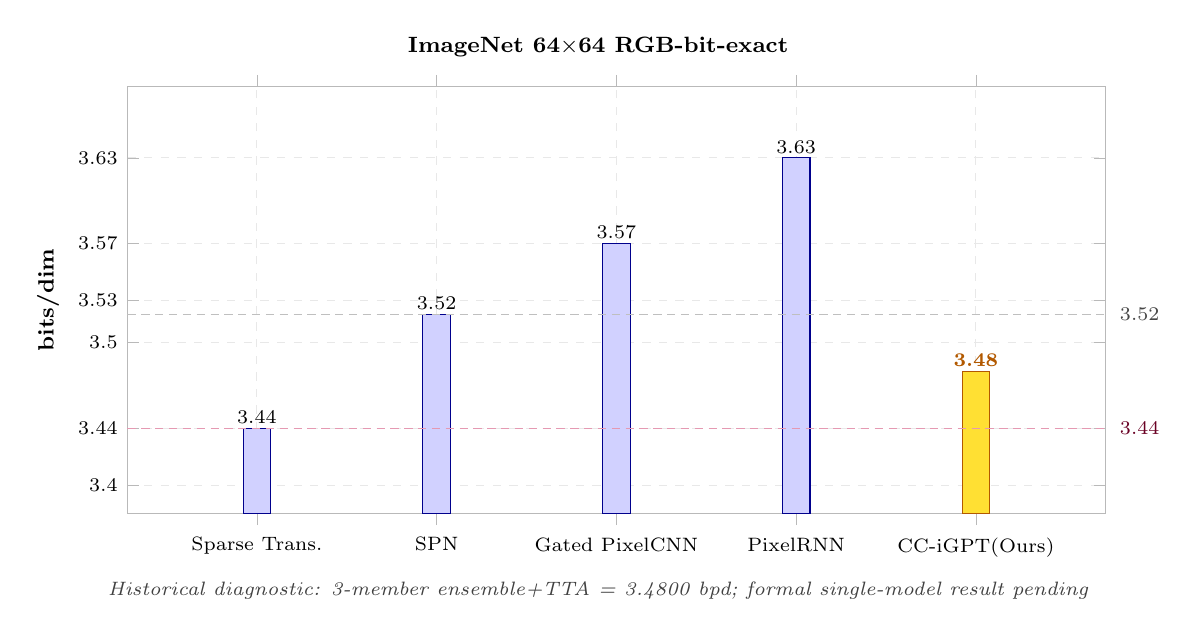
\begin{tikzpicture}[font=\footnotesize]
\begin{axis}[
    width=14cm, height=7cm,
    ybar,
    bar width=10pt,
    enlarge x limits=0.18,
    ymin=3.38, ymax=3.68,
    ytick={3.40,3.44,3.50,3.53,3.57,3.63},
    ylabel={\textbf{bits/dim}\ },
    ylabel near ticks,
    xtick={SparseTrans, SPN, GatedPCNN, PixelRNN, Ours},
    symbolic x coords={SparseTrans, SPN, GatedPCNN, PixelRNN, Ours},
    xticklabels={Sparse Trans., SPN, Gated PixelCNN, PixelRNN, CC-iGPT(Ours)},
    xticklabel style={font=\scriptsize, yshift=-1pt},
    yticklabel style={font=\scriptsize},
    axis line style={gray!55},
    tick style={gray!55},
    grid=major,
    grid style={dashed, gray!18, line width=0.3pt},
    major grid style={dashed, gray!18},
    clip=false,
]

% 前4个蓝色柱子（学术 baseline，升序）
\addplot[draw=blue!55!black, fill=blue!18, bar shift=0pt] coordinates {
    (SparseTrans, 3.44)
    (SPN,         3.52)
    (GatedPCNN,   3.57)
    (PixelRNN,    3.63)
};

% 第5个橘黄柱子（Ours，历史 ensemble+TTA 3.4800）
\addplot[draw=orange!70!black, fill=orange!30!yellow!80, bar shift=0pt] coordinates {
    (Ours, 3.4800)
};

% --- 参考线 1：SPN 3.52（coarse-to-fine 最近邻）---
\draw[densely dashed, gray!50, line width=0.4pt]
    ({rel axis cs:0,0}|-{axis cs:SparseTrans,3.52})
    -- ({rel axis cs:1,0}|-{axis cs:SparseTrans,3.52});
\node[font=\scriptsize, gray!55!black, anchor=west]
    at ({rel axis cs:1.005,0}|-{axis cs:SparseTrans,3.52}) {3.52};

% --- 参考线 2：Sparse Transformer 3.44（Ours 追的目标）---
\draw[densely dashed, purple!40, line width=0.4pt]
    ({rel axis cs:0,0}|-{axis cs:SparseTrans,3.44})
    -- ({rel axis cs:1,0}|-{axis cs:SparseTrans,3.44});
\node[font=\scriptsize, purple!55!black, anchor=west]
    at ({rel axis cs:1.005,0}|-{axis cs:SparseTrans,3.44}) {3.44};

% --- 柱顶标注 ---
\node[font=\scriptsize, align=center, yshift=4pt] at (axis cs:SparseTrans, 3.44) {3.44};
\node[font=\scriptsize, align=center, yshift=4pt] at (axis cs:SPN, 3.52) {3.52};
\node[font=\scriptsize, align=center, yshift=4pt] at (axis cs:GatedPCNN, 3.57) {3.57};
\node[font=\scriptsize, align=center, yshift=4pt] at (axis cs:PixelRNN, 3.63) {3.63};
\node[font=\scriptsize, align=center, orange!70!black, yshift=4pt] at (axis cs:Ours, 3.4800) {\textbf{3.48}};

\end{axis}

% --- 标题 ---
\node[font=\footnotesize\bfseries, anchor=south, yshift=3pt]
    at (current bounding box.north) {ImageNet 64$\times$64 RGB-bit-exact};

% --- 占位脚注 (ASCII only, pdflatex 可编译) ---
\node[font=\scriptsize\itshape, gray!50!black, anchor=north, yshift=-2pt]
    at (current bounding box.south)
    {Historical diagnostic: 3-member ensemble+TTA = 3.4800 bpd; formal single-model result pending};

\end{tikzpicture}
\end{document}

%
% 数据来源（AR 像素级，同口径 ImageNet 64x64 RGB bits/dim，越低越好）:
%   PixelRNN            3.63   van den Oord et al., ICML 2016
%   Gated PixelCNN      3.57   van den Oord et al., NeurIPS 2016
%   SPN (Subscale)      3.52   Menick & Kalchbrenner, ICLR 2019 (coarse-to-fine 最近邻)
%   Sparse Transformer  3.44   Child et al., 2019  ← 目标线
%   CC-iGPT (historical) 3.4800 本工作，IN64 v1 12ep，ensemble(best+SWA+EMA)+TTA hflip（4卡实测 2026-06-07）
%
% 历史实验结果 3.4800（diagnostic protocol：ensemble best/SWA/EMA + TTA hflip；单 ckpt best+TTA=3.4810）。
%   数值位于 SPN 3.52 与 Sparse Transformer 3.44 之间，但协议不同，不作正式优劣声明。
%   旧 ±0.1161 是 batch-level std，已作废；正式结果等待单 checkpoint/no-TTA 逐图重评。
\documentclass[tikz,border=8pt]{standalone}
\usepackage{tikz}
\usepackage{pgfplots}
\usepackage{amsmath,amssymb}
\pgfplotsset{compat=1.18}

\begin{document}
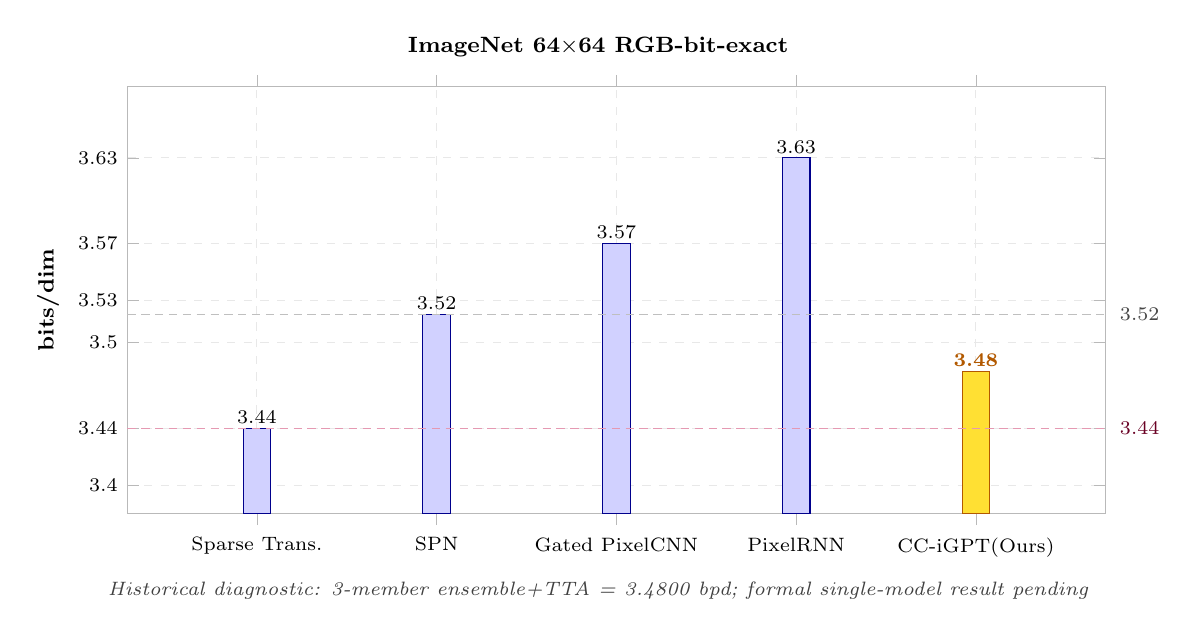
\begin{tikzpicture}[font=\footnotesize]
\begin{axis}[
    width=14cm, height=7cm,
    ybar,
    bar width=10pt,
    enlarge x limits=0.18,
    ymin=3.38, ymax=3.68,
    ytick={3.40,3.44,3.50,3.53,3.57,3.63},
    ylabel={\textbf{bits/dim}\ },
    ylabel near ticks,
    xtick={SparseTrans, SPN, GatedPCNN, PixelRNN, Ours},
    symbolic x coords={SparseTrans, SPN, GatedPCNN, PixelRNN, Ours},
    xticklabels={Sparse Trans., SPN, Gated PixelCNN, PixelRNN, CC-iGPT(Ours)},
    xticklabel style={font=\scriptsize, yshift=-1pt},
    yticklabel style={font=\scriptsize},
    axis line style={gray!55},
    tick style={gray!55},
    grid=major,
    grid style={dashed, gray!18, line width=0.3pt},
    major grid style={dashed, gray!18},
    clip=false,
]

% 前4个蓝色柱子（学术 baseline，升序）
\addplot[draw=blue!55!black, fill=blue!18, bar shift=0pt] coordinates {
    (SparseTrans, 3.44)
    (SPN,         3.52)
    (GatedPCNN,   3.57)
    (PixelRNN,    3.63)
};

% 第5个橘黄柱子（Ours，历史 ensemble+TTA 3.4800）
\addplot[draw=orange!70!black, fill=orange!30!yellow!80, bar shift=0pt] coordinates {
    (Ours, 3.4800)
};

% --- 参考线 1：SPN 3.52（coarse-to-fine 最近邻）---
\draw[densely dashed, gray!50, line width=0.4pt]
    ({rel axis cs:0,0}|-{axis cs:SparseTrans,3.52})
    -- ({rel axis cs:1,0}|-{axis cs:SparseTrans,3.52});
\node[font=\scriptsize, gray!55!black, anchor=west]
    at ({rel axis cs:1.005,0}|-{axis cs:SparseTrans,3.52}) {3.52};

% --- 参考线 2：Sparse Transformer 3.44（Ours 追的目标）---
\draw[densely dashed, purple!40, line width=0.4pt]
    ({rel axis cs:0,0}|-{axis cs:SparseTrans,3.44})
    -- ({rel axis cs:1,0}|-{axis cs:SparseTrans,3.44});
\node[font=\scriptsize, purple!55!black, anchor=west]
    at ({rel axis cs:1.005,0}|-{axis cs:SparseTrans,3.44}) {3.44};

% --- 柱顶标注 ---
\node[font=\scriptsize, align=center, yshift=4pt] at (axis cs:SparseTrans, 3.44) {3.44};
\node[font=\scriptsize, align=center, yshift=4pt] at (axis cs:SPN, 3.52) {3.52};
\node[font=\scriptsize, align=center, yshift=4pt] at (axis cs:GatedPCNN, 3.57) {3.57};
\node[font=\scriptsize, align=center, yshift=4pt] at (axis cs:PixelRNN, 3.63) {3.63};
\node[font=\scriptsize, align=center, orange!70!black, yshift=4pt] at (axis cs:Ours, 3.4800) {\textbf{3.48}};

\end{axis}

% --- 标题 ---
\node[font=\footnotesize\bfseries, anchor=south, yshift=3pt]
    at (current bounding box.north) {ImageNet 64$\times$64 RGB-bit-exact};

% --- 占位脚注 (ASCII only, pdflatex 可编译) ---
\node[font=\scriptsize\itshape, gray!50!black, anchor=north, yshift=-2pt]
    at (current bounding box.south)
    {Historical diagnostic: 3-member ensemble+TTA = 3.4800 bpd; formal single-model result pending};

\end{tikzpicture}
\end{document}

%
% 数据来源（AR 像素级，同口径 ImageNet 64x64 RGB bits/dim，越低越好）:
%   PixelRNN            3.63   van den Oord et al., ICML 2016
%   Gated PixelCNN      3.57   van den Oord et al., NeurIPS 2016
%   SPN (Subscale)      3.52   Menick & Kalchbrenner, ICLR 2019 (coarse-to-fine 最近邻)
%   Sparse Transformer  3.44   Child et al., 2019  ← 目标线
%   CC-iGPT (historical) 3.4800 本工作，IN64 v1 12ep，ensemble(best+SWA+EMA)+TTA hflip（4卡实测 2026-06-07）
%
% 历史实验结果 3.4800（diagnostic protocol：ensemble best/SWA/EMA + TTA hflip；单 ckpt best+TTA=3.4810）。
%   数值位于 SPN 3.52 与 Sparse Transformer 3.44 之间，但协议不同，不作正式优劣声明。
%   旧 ±0.1161 是 batch-level std，已作废；正式结果等待单 checkpoint/no-TTA 逐图重评。
\documentclass[tikz,border=8pt]{standalone}
\usepackage{tikz}
\usepackage{pgfplots}
\usepackage{amsmath,amssymb}
\pgfplotsset{compat=1.18}

\begin{document}
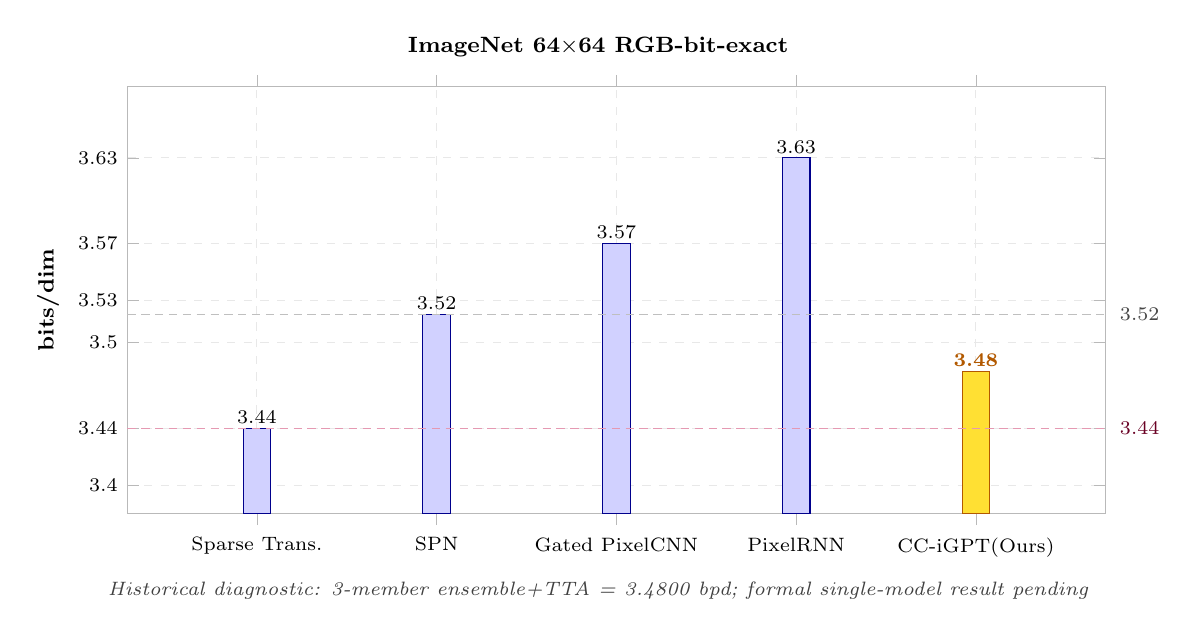
\begin{tikzpicture}[font=\footnotesize]
\begin{axis}[
    width=14cm, height=7cm,
    ybar,
    bar width=10pt,
    enlarge x limits=0.18,
    ymin=3.38, ymax=3.68,
    ytick={3.40,3.44,3.50,3.53,3.57,3.63},
    ylabel={\textbf{bits/dim}\ },
    ylabel near ticks,
    xtick={SparseTrans, SPN, GatedPCNN, PixelRNN, Ours},
    symbolic x coords={SparseTrans, SPN, GatedPCNN, PixelRNN, Ours},
    xticklabels={Sparse Trans., SPN, Gated PixelCNN, PixelRNN, CC-iGPT(Ours)},
    xticklabel style={font=\scriptsize, yshift=-1pt},
    yticklabel style={font=\scriptsize},
    axis line style={gray!55},
    tick style={gray!55},
    grid=major,
    grid style={dashed, gray!18, line width=0.3pt},
    major grid style={dashed, gray!18},
    clip=false,
]

% 前4个蓝色柱子（学术 baseline，升序）
\addplot[draw=blue!55!black, fill=blue!18, bar shift=0pt] coordinates {
    (SparseTrans, 3.44)
    (SPN,         3.52)
    (GatedPCNN,   3.57)
    (PixelRNN,    3.63)
};

% 第5个橘黄柱子（Ours，历史 ensemble+TTA 3.4800）
\addplot[draw=orange!70!black, fill=orange!30!yellow!80, bar shift=0pt] coordinates {
    (Ours, 3.4800)
};

% --- 参考线 1：SPN 3.52（coarse-to-fine 最近邻）---
\draw[densely dashed, gray!50, line width=0.4pt]
    ({rel axis cs:0,0}|-{axis cs:SparseTrans,3.52})
    -- ({rel axis cs:1,0}|-{axis cs:SparseTrans,3.52});
\node[font=\scriptsize, gray!55!black, anchor=west]
    at ({rel axis cs:1.005,0}|-{axis cs:SparseTrans,3.52}) {3.52};

% --- 参考线 2：Sparse Transformer 3.44（Ours 追的目标）---
\draw[densely dashed, purple!40, line width=0.4pt]
    ({rel axis cs:0,0}|-{axis cs:SparseTrans,3.44})
    -- ({rel axis cs:1,0}|-{axis cs:SparseTrans,3.44});
\node[font=\scriptsize, purple!55!black, anchor=west]
    at ({rel axis cs:1.005,0}|-{axis cs:SparseTrans,3.44}) {3.44};

% --- 柱顶标注 ---
\node[font=\scriptsize, align=center, yshift=4pt] at (axis cs:SparseTrans, 3.44) {3.44};
\node[font=\scriptsize, align=center, yshift=4pt] at (axis cs:SPN, 3.52) {3.52};
\node[font=\scriptsize, align=center, yshift=4pt] at (axis cs:GatedPCNN, 3.57) {3.57};
\node[font=\scriptsize, align=center, yshift=4pt] at (axis cs:PixelRNN, 3.63) {3.63};
\node[font=\scriptsize, align=center, orange!70!black, yshift=4pt] at (axis cs:Ours, 3.4800) {\textbf{3.48}};

\end{axis}

% --- 标题 ---
\node[font=\footnotesize\bfseries, anchor=south, yshift=3pt]
    at (current bounding box.north) {ImageNet 64$\times$64 RGB-bit-exact};

% --- 占位脚注 (ASCII only, pdflatex 可编译) ---
\node[font=\scriptsize\itshape, gray!50!black, anchor=north, yshift=-2pt]
    at (current bounding box.south)
    {Historical diagnostic: 3-member ensemble+TTA = 3.4800 bpd; formal single-model result pending};

\end{tikzpicture}
\end{document}

%
% 数据来源（AR 像素级，同口径 ImageNet 64x64 RGB bits/dim，越低越好）:
%   PixelRNN            3.63   van den Oord et al., ICML 2016
%   Gated PixelCNN      3.57   van den Oord et al., NeurIPS 2016
%   SPN (Subscale)      3.52   Menick & Kalchbrenner, ICLR 2019 (coarse-to-fine 最近邻)
%   Sparse Transformer  3.44   Child et al., 2019  ← 目标线
%   CC-iGPT (historical) 3.4800 本工作，IN64 v1 12ep，ensemble(best+SWA+EMA)+TTA hflip（4卡实测 2026-06-07）
%
% 历史实验结果 3.4800（diagnostic protocol：ensemble best/SWA/EMA + TTA hflip；单 ckpt best+TTA=3.4810）。
%   数值位于 SPN 3.52 与 Sparse Transformer 3.44 之间，但协议不同，不作正式优劣声明。
%   旧 ±0.1161 是 batch-level std，已作废；正式结果等待单 checkpoint/no-TTA 逐图重评。
\documentclass[tikz,border=8pt]{standalone}
\usepackage{tikz}
\usepackage{pgfplots}
\usepackage{amsmath,amssymb}
\pgfplotsset{compat=1.18}

\begin{document}
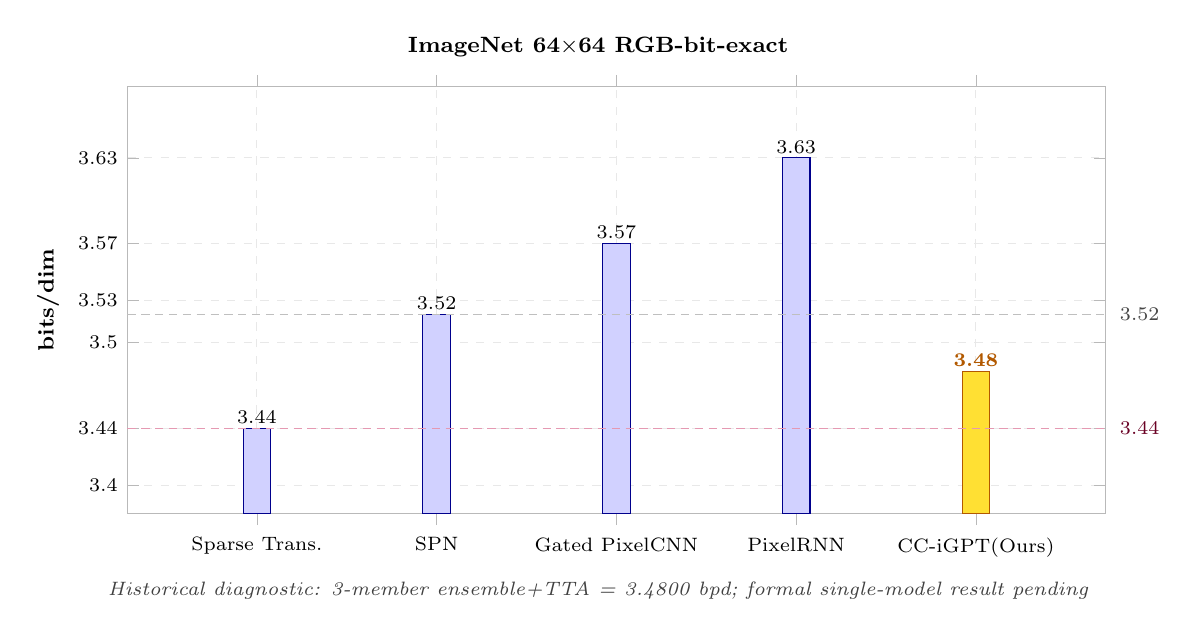
\begin{tikzpicture}[font=\footnotesize]
\begin{axis}[
    width=14cm, height=7cm,
    ybar,
    bar width=10pt,
    enlarge x limits=0.18,
    ymin=3.38, ymax=3.68,
    ytick={3.40,3.44,3.50,3.53,3.57,3.63},
    ylabel={\textbf{bits/dim}\ },
    ylabel near ticks,
    xtick={SparseTrans, SPN, GatedPCNN, PixelRNN, Ours},
    symbolic x coords={SparseTrans, SPN, GatedPCNN, PixelRNN, Ours},
    xticklabels={Sparse Trans., SPN, Gated PixelCNN, PixelRNN, CC-iGPT(Ours)},
    xticklabel style={font=\scriptsize, yshift=-1pt},
    yticklabel style={font=\scriptsize},
    axis line style={gray!55},
    tick style={gray!55},
    grid=major,
    grid style={dashed, gray!18, line width=0.3pt},
    major grid style={dashed, gray!18},
    clip=false,
]

% 前4个蓝色柱子（学术 baseline，升序）
\addplot[draw=blue!55!black, fill=blue!18, bar shift=0pt] coordinates {
    (SparseTrans, 3.44)
    (SPN,         3.52)
    (GatedPCNN,   3.57)
    (PixelRNN,    3.63)
};

% 第5个橘黄柱子（Ours，历史 ensemble+TTA 3.4800）
\addplot[draw=orange!70!black, fill=orange!30!yellow!80, bar shift=0pt] coordinates {
    (Ours, 3.4800)
};

% --- 参考线 1：SPN 3.52（coarse-to-fine 最近邻）---
\draw[densely dashed, gray!50, line width=0.4pt]
    ({rel axis cs:0,0}|-{axis cs:SparseTrans,3.52})
    -- ({rel axis cs:1,0}|-{axis cs:SparseTrans,3.52});
\node[font=\scriptsize, gray!55!black, anchor=west]
    at ({rel axis cs:1.005,0}|-{axis cs:SparseTrans,3.52}) {3.52};

% --- 参考线 2：Sparse Transformer 3.44（Ours 追的目标）---
\draw[densely dashed, purple!40, line width=0.4pt]
    ({rel axis cs:0,0}|-{axis cs:SparseTrans,3.44})
    -- ({rel axis cs:1,0}|-{axis cs:SparseTrans,3.44});
\node[font=\scriptsize, purple!55!black, anchor=west]
    at ({rel axis cs:1.005,0}|-{axis cs:SparseTrans,3.44}) {3.44};

% --- 柱顶标注 ---
\node[font=\scriptsize, align=center, yshift=4pt] at (axis cs:SparseTrans, 3.44) {3.44};
\node[font=\scriptsize, align=center, yshift=4pt] at (axis cs:SPN, 3.52) {3.52};
\node[font=\scriptsize, align=center, yshift=4pt] at (axis cs:GatedPCNN, 3.57) {3.57};
\node[font=\scriptsize, align=center, yshift=4pt] at (axis cs:PixelRNN, 3.63) {3.63};
\node[font=\scriptsize, align=center, orange!70!black, yshift=4pt] at (axis cs:Ours, 3.4800) {\textbf{3.48}};

\end{axis}

% --- 标题 ---
\node[font=\footnotesize\bfseries, anchor=south, yshift=3pt]
    at (current bounding box.north) {ImageNet 64$\times$64 RGB-bit-exact};

% --- 占位脚注 (ASCII only, pdflatex 可编译) ---
\node[font=\scriptsize\itshape, gray!50!black, anchor=north, yshift=-2pt]
    at (current bounding box.south)
    {Historical diagnostic: 3-member ensemble+TTA = 3.4800 bpd; formal single-model result pending};

\end{tikzpicture}
\end{document}
